\oldpage{418}
\begin{figure}[H]
  \centering
  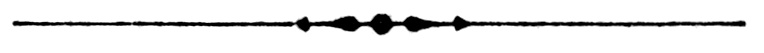
\includegraphics{pages/illustrations/arrow_bullet_divider.jpg}
\end{figure}
\section*{Caution---An Attempt at Fraud.}

\SectionStartWords{On} making inquiry this morning at one of our first class book-seller's
for the English edition of ``Gregory's Chemistry,'' I was offered a
book which, on examination, I found to be curiously mutilated, viz:
the title page had a strip of white paper very neatly pasted over a
portion of it, which piece of paper upon close examination I found answered
the purpose of concealing the fact that the book was published
under the editorial care of one \emph{J.~Milton Sanders}, \md{} To this attempt
at concealment on the part of the book-seller or publisher (I care not
which), I feel it my duty to call the attention of the profession. I also
wish to notice the fact that those having the work to sell feel ashamed
of the so-called ``reprint'' of Prof.~Gregory's excellent work, yet are
attempting by this contemptible trick to avoid the influence of the
many severe, though just notices the work as edited by Sanders has received.
I would call the attention of the reader to the notices on pages
\typo{82--84}{82-3 4} and 232--3 of the present volume of the \ThisJournal{College Journal}.\hfill{}J.~F.~J.\quad

\plainbreak{1}

\textsc{Note}---Although I was prepared for almost any attempt at deceiving
the profession by the American Editor of Gregory's Chemistry, I was
not inclined to allow a statement like the above to rest solely on the
authority of the writer of the above communication, every way worthy
of entire belief as I know his statement to be; hence I went to the
book store where this work was offered for sale, and on examination
I found it was the old edition which W.~H.~Derby~\& Co.\ of this city,
had copyrighted.

The honorable proprietor of the book store viewed this attempt at
deception as any honorable, high-minded man must, and offered his
assistance in determining the extent to which the mutilation had been
carried and the fraud perpetrated.

If the repeated instances of deception of the American editor and
the publishers of Gregory's Chemistry should lead the readers of the
\ThisJournal{College Journal} to renewed interest in the book, I would refer them
to the \booktitle{American Journal of Pharmacy} for Jan.\ last, page 89 \foreign{et Seq.}\ 
and to the \booktitle{American Journal of Arts and Sciences} for March last, for
a more extended reference to this subject. We should feel it our duty
to say much more in regard to these frequent attempts at deception
on the part of the individual referred to above, were we not aware that
our readers are fully acquainted with the character of the party engaged
in the fraud.\hfill{}C.
\endinput
